\begin{titlepage}
\begin{center}
  \vspace*{\stretch{0.5}}

  \large % Default size for the title page

  {\Huge\textsc{Categorical Realizability}\par}

  \vspace{\stretch{0.2}}

  by

  \vspace{\stretch{0.2}}

  {\huge\textsc{Tom de Jong}}

  \vspace{\stretch{0.5}}

  {\Large{Lecture notes and exercises for the\\
      \textsc{Midlands Graduate School (MGS)}}} \\
  \vspace{\stretch{0.1}}
  8--12 April 2024, Leicester, UK

  \vspace{\stretch{1}}

  % \begingroup
  % \tikzset{every picture/.style={color=Gray!90!Black}}
  % \begin{tikzcd}
  %   0 & 1 & 2 & 3 & \ldots \\
  %   & & \bot \ar[ull,no head] \ar[ul,no head] \ar[u,no head] \ar[ur, no head] \ar[urr, no head]
  % \end{tikzcd}
  % \endgroup

  \begingroup
  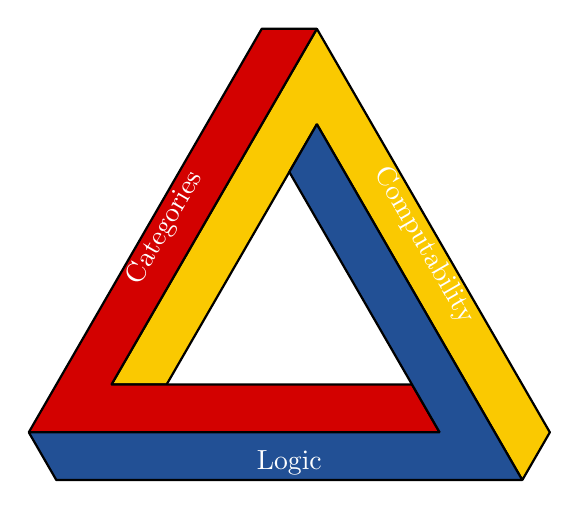
\begin{tikzpicture}[scale=1, line join=bevel]

  \definecolor{mondrianYellow}{RGB}{250,201,1}
  \definecolor{mondrianBlue}{RGB}{34,80,149}
  \definecolor{mondrianRed}{RGB}{211,1,0}

  % \a and \b are two macros defining characteristic
  % dimensions of the Penrose triangle.
  \pgfmathsetmacro{\a}{1.8}
  \pgfmathsetmacro{\b}{0.7}

  \tikzset{%
    apply style/.code     = {\tikzset{#1}},
    triangle_edges/.style = {thick,draw=black}
  }

  \foreach \theta/\facestyle/\city/\al\/\ang in {%
    %   0/{triangle_edges, fill = gray!50}/\hphantom{1pt}Computability/below/-60,
    % 120/{triangle_edges, fill = gray!25}/Categories/below/60,
    % 240/{triangle_edges, fill = gray!90}/\raisebox{5pt}{Logic}/above/0}
      0/{triangle_edges, fill = mondrianYellow}/\hphantom{1pt}Computability/below/-60,
    120/{triangle_edges, fill = mondrianRed}/Categories/below/60,
    240/{triangle_edges, fill = mondrianBlue}/\raisebox{5pt}{Logic}/above/0}
    {
    \begin{scope}[rotate=\theta]
      \draw[apply style/.expand once=\facestyle]
        ({-sqrt(3)/2*\a},{-0.5*\a})                   --
        ++  (-\b,0)                                   --
          ({0.5*\b},{\a+3*sqrt(3)/2*\b})                --node[\al=-5pt,rotate=\ang,text=White]{\city} % higher point
          ({sqrt(3)/2*\a+2.5*\b},{-.5*\a-sqrt(3)/2*\b}) -- % rightmost point
        ++({-.5*\b},-{sqrt(3)/2*\b})                    -- % lower point
          ({0.5*\b},{\a+sqrt(3)/2*\b})                  --
        cycle;
      \end{scope}
    }
   \end{tikzpicture}
  \endgroup

  \vfill

  \flushright
  {\normalsize{School of Computer Science \\
  University of Nottingham \\
  January--March 2024}}

\end{center}
\end{titlepage}

%%% Local Variables:
%%% mode: latexmk
%%% TeX-master: "../main"
%%% End: